\documentclass[xetex]{beamer}
\usepackage{fontspec}
\usepackage{bytefield}

\title{Automatisk upptäckt av strukturer för binära nätverksprotokoll}
\author{Fredrik Appelros \& Carl Ekerot}
\date

\setbeamertemplate{navigation symbols}{}
\renewcommand*{\thefootnote}{\fnsymbol{footnote}}

% Introducera problemet - applikationer
% Tidigare försök
% Kort om vårt angreppssätt
% Hitta pakettyper (2 delar)
% Klustring
% Förfining av typindelning
% Fältanalys (bygger på bytefördelningar)
% Olika fälttyper
% Tillståndsdiagram
% Resultat - jämförelse mellan definition och inferens
% Begränsningar

\begin{document}
    \frame{\titlepage}
    
    % Introduktion
    \begin{frame}
        \frametitle{Binära nätveksprotokoll}
        \begin{columns}[t]
            \begin{column}[T]{8cm}
                \begin{itemize}
                    \item Språk för mjukvara eller hårdvara
                    \item Binärt kodat -- svårläst utan specifikation
                    \item Byggs upp av fält som representerar nummer, flaggor,
                        data osv.
                    \item Exempel: DNS, SMB, RTP, DHCP, \ldots
                \end{itemize}
            \end{column}
            \begin{column}[T]{6cm}
                \begin{bytefield}[bitwidth=0.56em]{16}
                    \bitheader{0, 16}\\
                    \wordbox{1}{\texttt{1000011010010000}}\\
                    \bitbox{1}{\texttt{1}}
                    \bitbox{4}{\texttt{0000}}
                    \bitbox{1}{\texttt{0}}
                    \bitbox{1}{\texttt{0}}
                    \bitbox{1}{\texttt{1}}
                    \bitbox{1}{\texttt{1}}
                    \bitbox{3}{\texttt{000}}
                    \bitbox{4}{\texttt{0000}}\\
                    \wordbox{1}{\texttt{0000000000000001}}\\
                    \wordbox{1}{\texttt{0000000000000010}}\\
                    \wordbox{1}{\texttt{0000000000000001}}\\
                    \wordbox{1}{\texttt{0000000000000000}}
                \end{bytefield}
            \end{column}
        \end{columns}
    \end{frame}
    \begin{frame}
        \frametitle{Slutna protokoll}
        \begin{itemize}
            \item Ett protokoll kan ha \emph{öppen} eller \emph{sluten}
                specifikation
            \item Slutet protokoll $\Rightarrow$ svårt att tyda meddelanden
            \item Proprietära eller odokumenterade
            \item Exempel: Skype, (tidigare) SMB
        \end{itemize}
        \vskip20pt
        Varför avkoda slutna protokoll?
        \begin{enumerate}
            \item Interoperabilitet (SMB)
            \item QoS
        \end{enumerate}
    \end{frame}
    \begin{frame}
        \frametitle{Tidigare försök}
        Discoverer, Microsoft (2005)
        \begin{itemize}
            \item Arbetar på nätverksdumpar (lagrad nätverkstrafik)
            \item Delar upp meddelanden i textuell och binär data
            \item Försöker hitta meddelandetyper
        \end{itemize}
        \vskip20pt
        Dispatcher, UC Berkeley (2012)
        \begin{itemize}
            \item Övervakar exekveringstillstånd
            \item Jämför nätverkstrafik med data i minnet
            \item Kräver mjukvaran/hårdvaran som använder protokollet
        \end{itemize}
    \end{frame}

    % Vår approach
    \begin{frame}
        \frametitle{Vårt angreppssätt}
        Input: Nätverksdump (pcap)\\
        Metod:
        \begin{enumerate}
            \item Identifiera meddelandetyper
                \begin{itemize}
                    \item Statistisk analys -- \emph{klustring}
                    \item Förfining -- hitta vad som definierar en meddelandetyp
                \end{itemize}
            \item Identifiera fält
                \begin{itemize}
                    \item Statistisk analys -- identifiera bytevärdesdistributioner
                    \item Identifiera fält specifika för strömmar och anslutningar
                    \item Hitta längdfält
                \end{itemize}
            \item Bygg tillståndsdiagram
                \begin{itemize}
                    \item Vilka meddelandetyper kan följa ett visst meddelande?
                \end{itemize}
        \end{enumerate}
    \end{frame}
    
    % Klustring
    \begin{frame}
        \frametitle{Hitta meddelandetyper}
        \begin{columns}[t]
            \begin{column}[T]{6cm}
                \begin{itemize}
                    \item Antagande: Liknande data $\Leftrightarrow$ samma meddelandetyp
                    \item Klustring: Gruppera datapunkter m.a.p. egendefinierade egenskaper
                        för varje datapunkt
                    \item Använda resultat från klustring för att hitta de bytes som
                        definierar ett meddelandes typ
                \end{itemize}
            \end{column}
            \begin{column}[T]{6cm}
                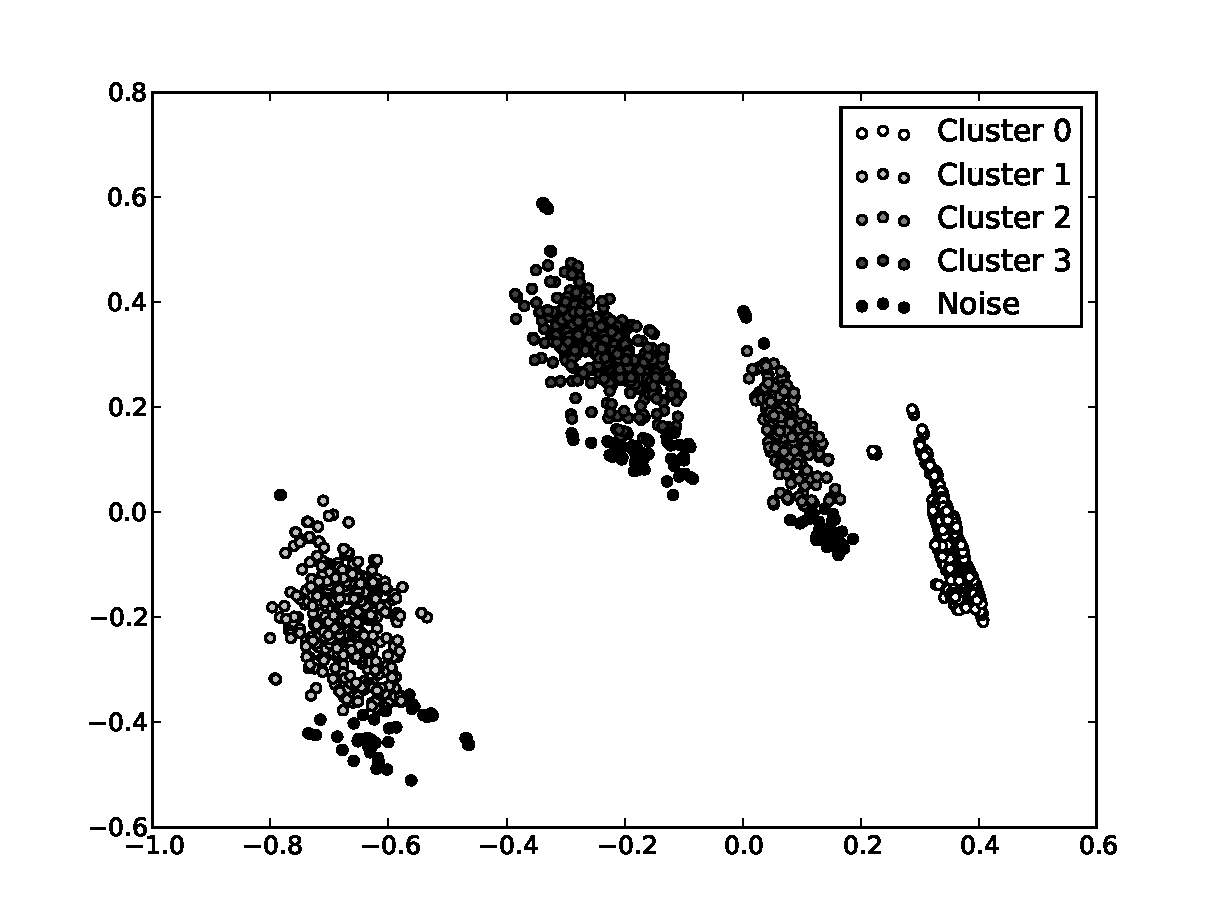
\includegraphics[height=4.5cm]{img/dbscan_dns.pdf}
            \end{column}
        \end{columns}
    \end{frame}
    \begin{frame}
        \frametitle{Hitta meddelandetyper -- Klustring}
        Problem:
        \begin{itemize}
            \item Okänt antal kluster (meddelandetyper)
            \item Varierande \emph{täthet} bland kluster
        \end{itemize}
        Lösning: \textbf{OPTICS}, \scriptsize{
            \emph{\underline{O}rdering \underline{P}oints \underline{T}o
                  \underline{I}dentify the \underline{C}lustering 
                  \underline{S}tructure}}
        \vskip20pt
        \begin{columns}[t]
            \begin{column}[T]{6cm}
                \begin{itemize}
                    \item \emph{Densitetsbaserad} klustringsalgoritm
                    \item Hittar kluster med olika täthet
                    \item Behöver ej fördefinierat antal kluster som parameter
                \end{itemize}
            \end{column}
            \begin{column}[T]{6cm}
                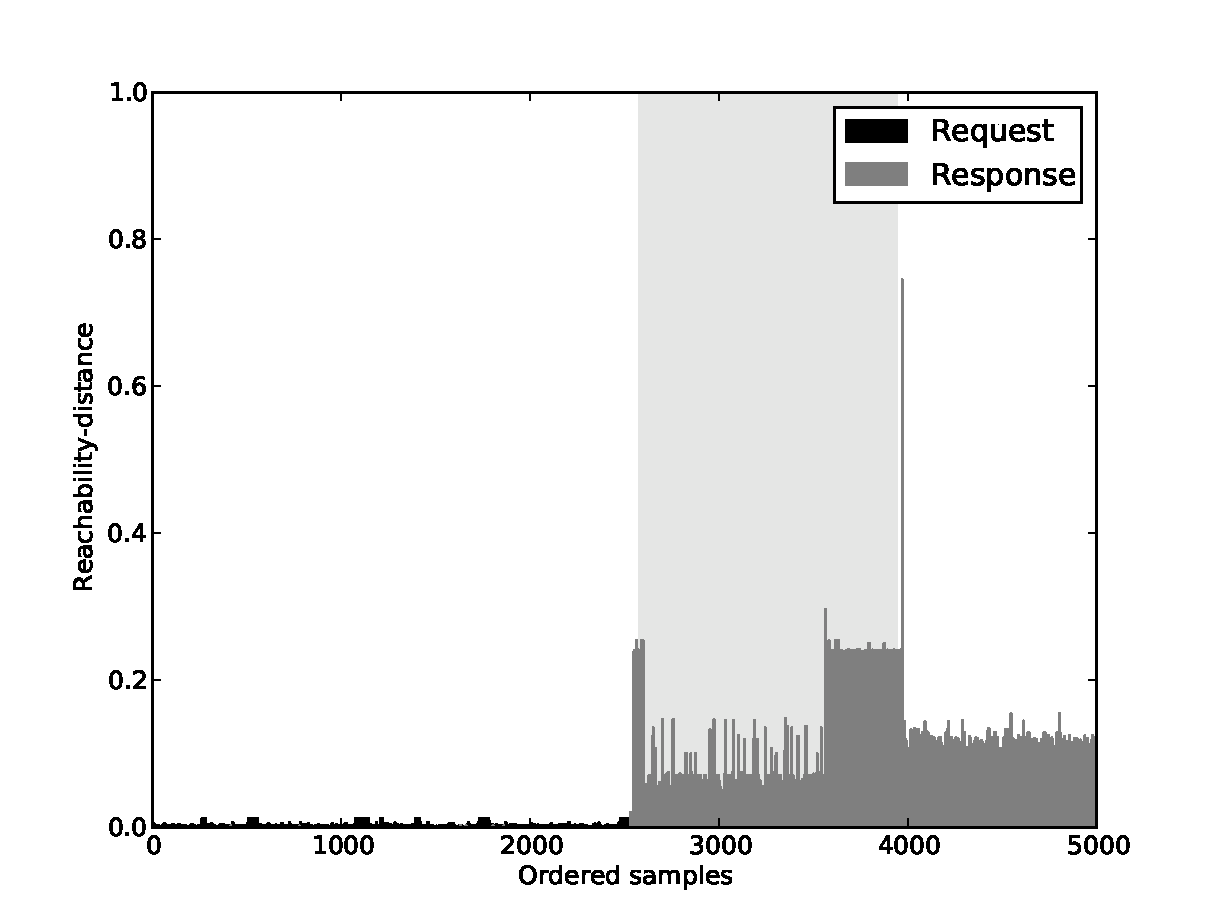
\includegraphics[height=4.5cm]{img/hierextr.pdf}
            \end{column}
        \end{columns}
    \end{frame}
    \begin{frame}
        \frametitle{Hitta meddelandetyper -- Klustring (forts.)}
        Egenskaper: Vektor $\{f_1, f_2, ..., f_n\}$
        \begin{itemize}
            \item $n$: Längsta meddelandets längd
            \item $f_i$: Sannolikhet för att bytevärdet på position $i$ i
                meddelandet är det värdet som det är.
        \end{itemize}
        \vskip20pt
        Problem: Hög dimensionalitet \\
        Lösning: \textbf{PCA}, \scriptsize{\underline{P}rincipal
            \underline{C}omponent \underline{A}nalysis}
    \end{frame}
    \begin{frame}
        \frametitle{Hitta meddelandetyper -- Förfining}
        \begin{itemize}
            \item \emph{Typ-bytes}: Bytes som bestämmer ett meddelandes typ \\
            \item Antagande: Om det finns typ-bytes så kommer de oftast ha
                samma värde inom kluster \\
            \item \emph{Completeness}: Hög om många datapunkter av en viss
                sann typ ligger inom samma kluster
        \end{itemize}
        \vskip20pt
        \textbf{Metod}: För varje byte-position, dela upp alla meddelanden
        efter de värden som byten antar. Har indelningen hög completeness mot
        OPTICS-klustringen: \underline{möjlig typ-byte}
    \end{frame}

    % Fält
    \begin{frame}
        \frametitle{Protokollens fält}
        \begin{itemize}
            \item Lagrar data som är intressant för protokollet
            \item Ligger ofta justerade efter 1, 2 eller 4 bytes
            \item Fälttyper vi observerat:
                \begin{itemize}
                    \item Konstanta fält
                    \item Flaggfält
                    \item Uniformt fördelade fält
                    \item Nummerfält
                    \item Inkrementella fält
                    \item Längdfält
                \end{itemize}
            \item Många fälttyper har speciell fördelning av bytevärden
        \end{itemize}
    \end{frame}

    % Något om hur vi kör vår klassificering

    \begin{frame}
        \frametitle{Konstanta fält}
        \begin{columns}[t]
            \begin{column}[T]{6cm}
                \begin{itemize}
                    \item Antar bara ett värde för alla meddelanden
                    \item Kan vara konstant globalt, inom ström, inom
                        anslutning eller inom typ
                    \item Lätt att klassificera
                \end{itemize}
            \end{column}
            \begin{column}[T]{6cm}
                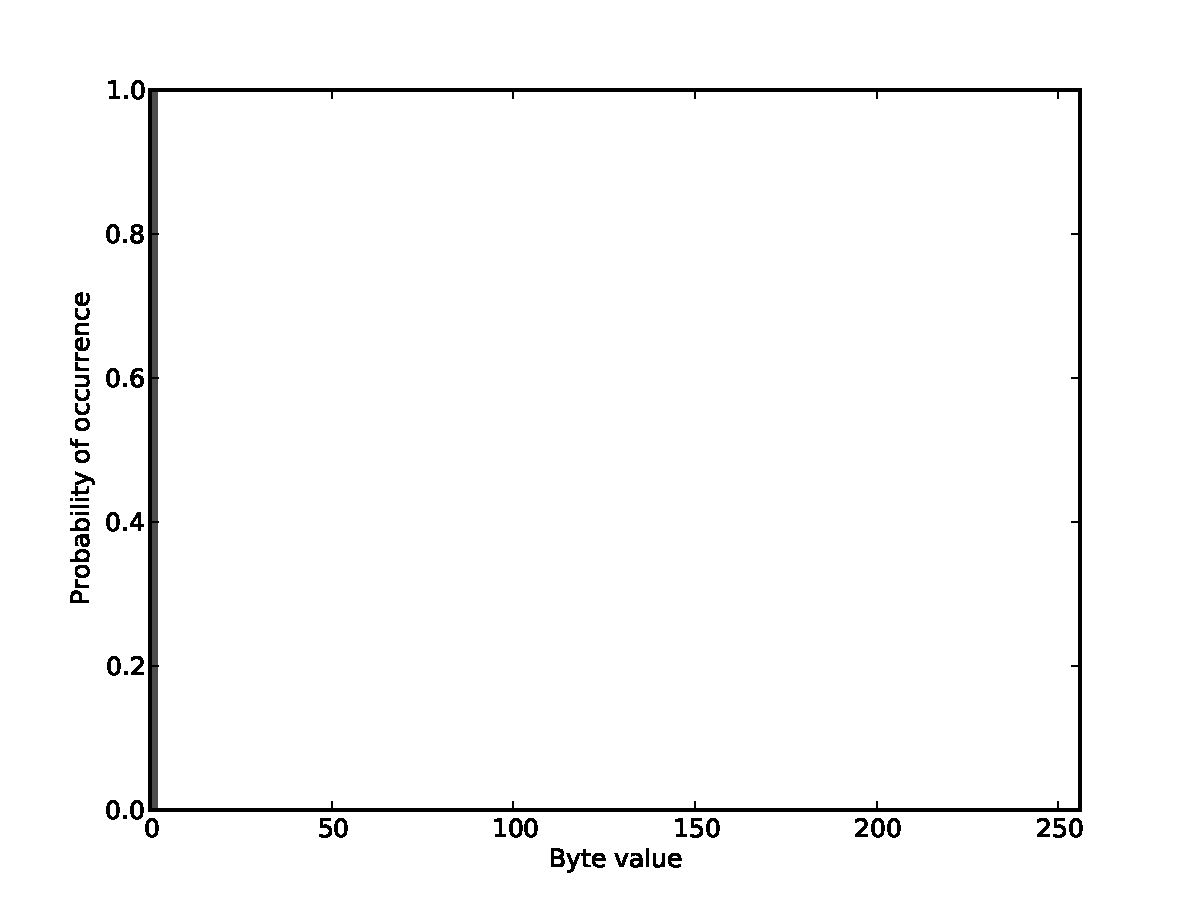
\includegraphics[height=5cm]{img/const_one.pdf}
            \end{column}
        \end{columns}
    \end{frame}
    \begin{frame}
        \frametitle{Flaggfält}
        \begin{columns}[t]
            \begin{column}[T]{6cm}
                \begin{itemize}
                    \item Antar fåtal värden för alla meddelanden
                    \item Klassificerar som flaggfält om fält antar minst
                        två värden men mindre värden än en övre gräns
                \end{itemize}
            \end{column}
            \begin{column}[T]{6cm}
                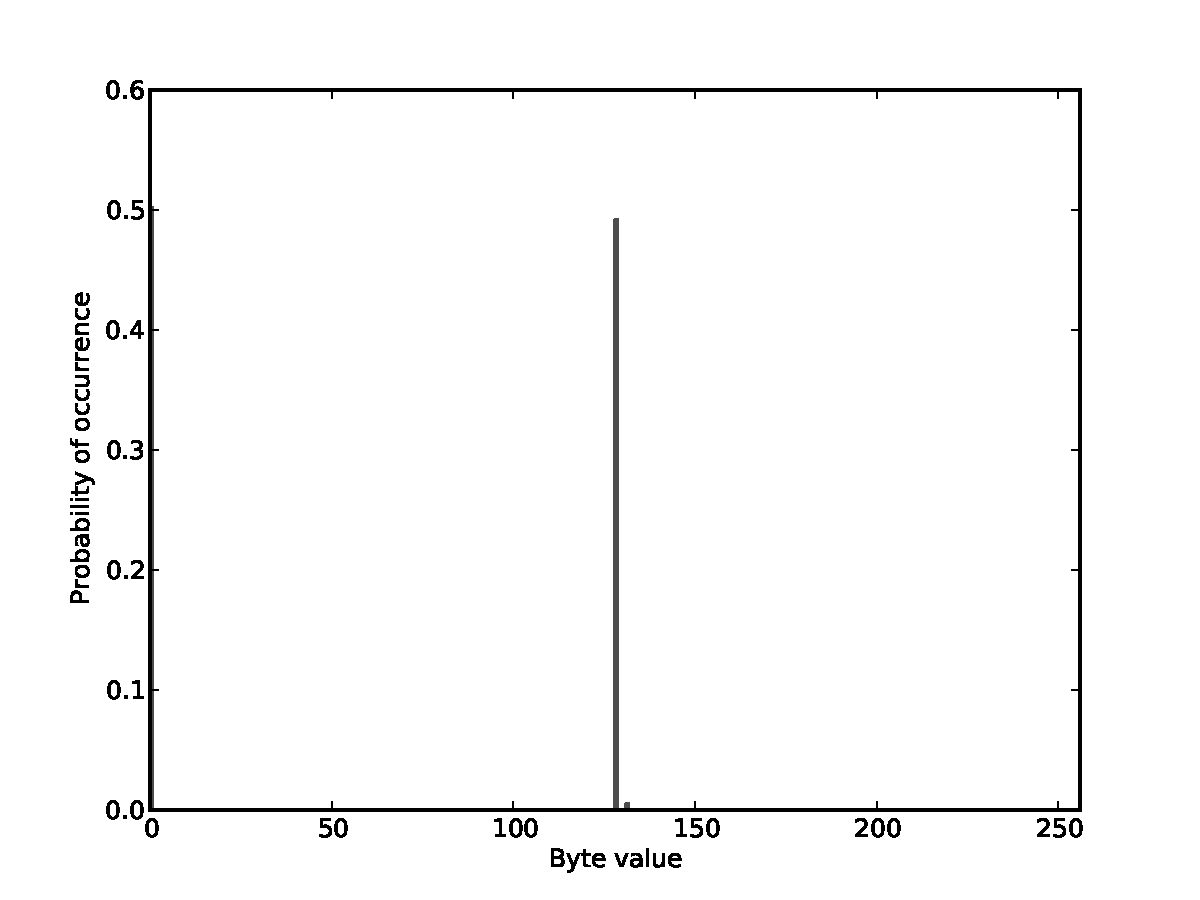
\includegraphics[height=5cm]{img/flag.pdf}
            \end{column}
        \end{columns}
    \end{frame}
    \begin{frame}
        \frametitle{Uniformt fördelade fält}
        \begin{columns}[t]
            \begin{column}[T]{6cm}
                \begin{itemize}
                    \item Uniform fördelning: Vanlig för slumptal
                    \item Vanlig för genererade värden så som ID:n
                    \item Klassificerar som uniformt om avstånd till 
                        rektangulär- fördelning är låg
                \end{itemize}
            \end{column}
            \begin{column}[T]{6cm}
                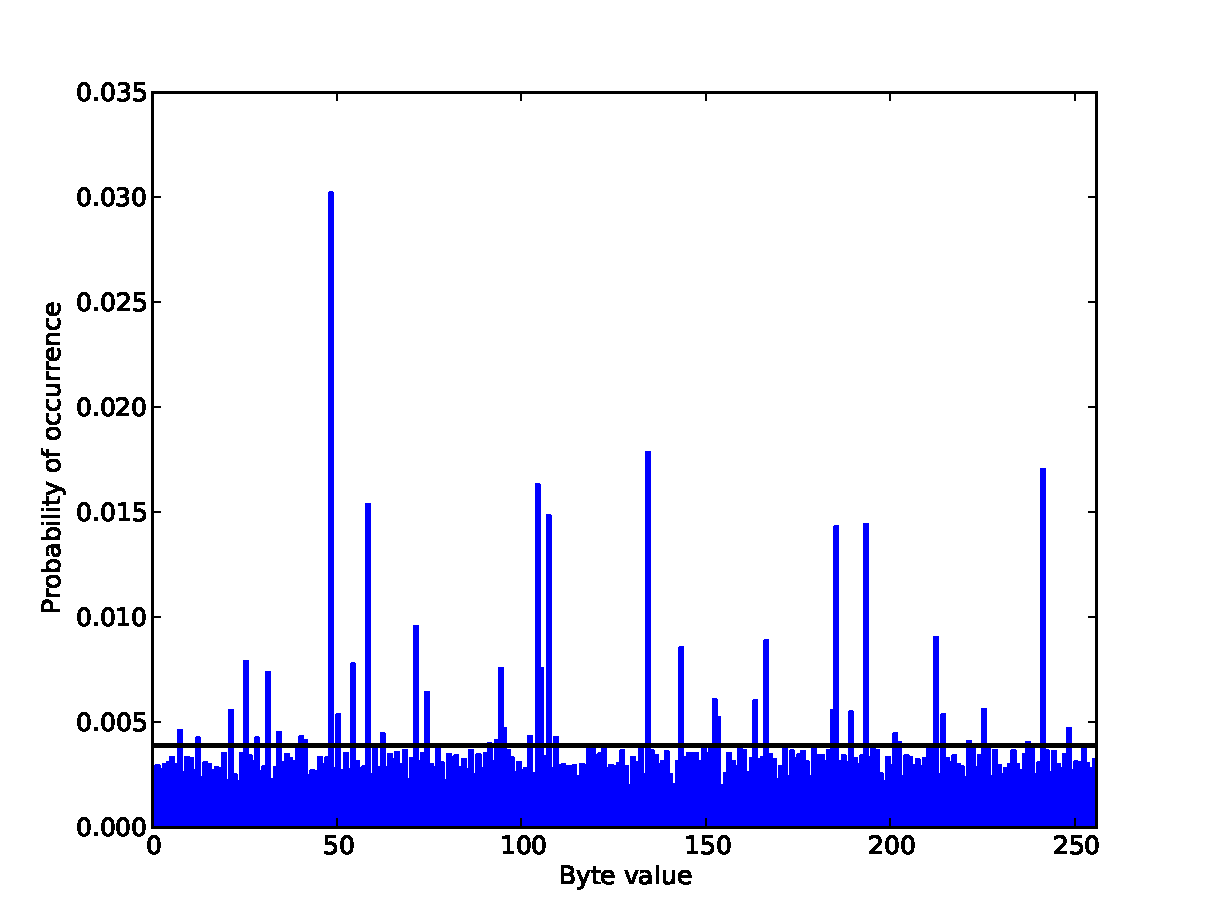
\includegraphics[height=5cm]{img/uniform.pdf}
            \end{column}
        \end{columns}
    \end{frame}
    \begin{frame}
        \frametitle{Nummerfält}
        \begin{columns}[t]
            \begin{column}[T]{6cm}
                \begin{itemize}
                    \item Fält som innehåller nummer, t.ex. antal
                    \item Observation: Normalfördelade
                    \item Klassificerar som nummerfält om vi kan få avståndet
                        till någon normalfördelningskurva att understiga ett
                        visst värde
                \end{itemize}
            \end{column}
            \begin{column}[T]{6cm}
                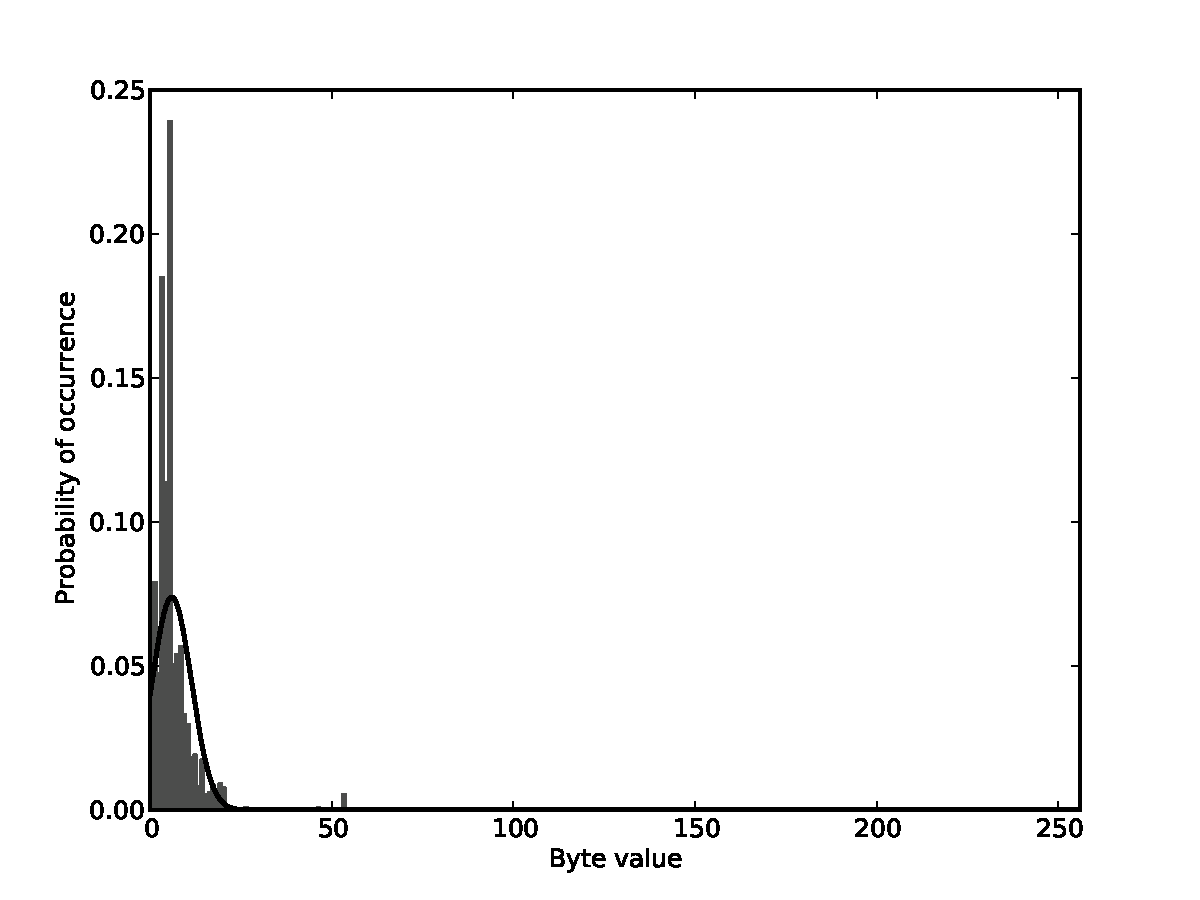
\includegraphics[height=5cm]{img/number.pdf}
            \end{column}
        \end{columns}
    \end{frame}
    \begin{frame}
        \frametitle{Inkrementella fält}
        \begin{itemize}
            \item Bytevärdesdistribution är ointressant
            \item Kan bara upptäckas inom ström eller anslutning
            \item Exempel: Sekvensnummer, räknare, tid
            \item Klassificerar som inkrementellt fält om dess värde
                oftast\footnote{Efter 255 kommer 0} är ökande genom
                ström/anslutning
        \end{itemize}
    \end{frame}
    \begin{frame}
        \frametitle{Längdfält}
        \begin{columns}[t]
            \begin{column}[T]{6cm}
                \begin{itemize}
                    \item Bestämmer längd på något fält inom meddelande
                    \item Observation: Värde i längdfält är proportionellt
                        mot meddelandets längd
                    \item Problem: Segmentering
                    \item Lösning: RANSAC
                \end{itemize}
            \end{column}
            \begin{column}[T]{6cm}
                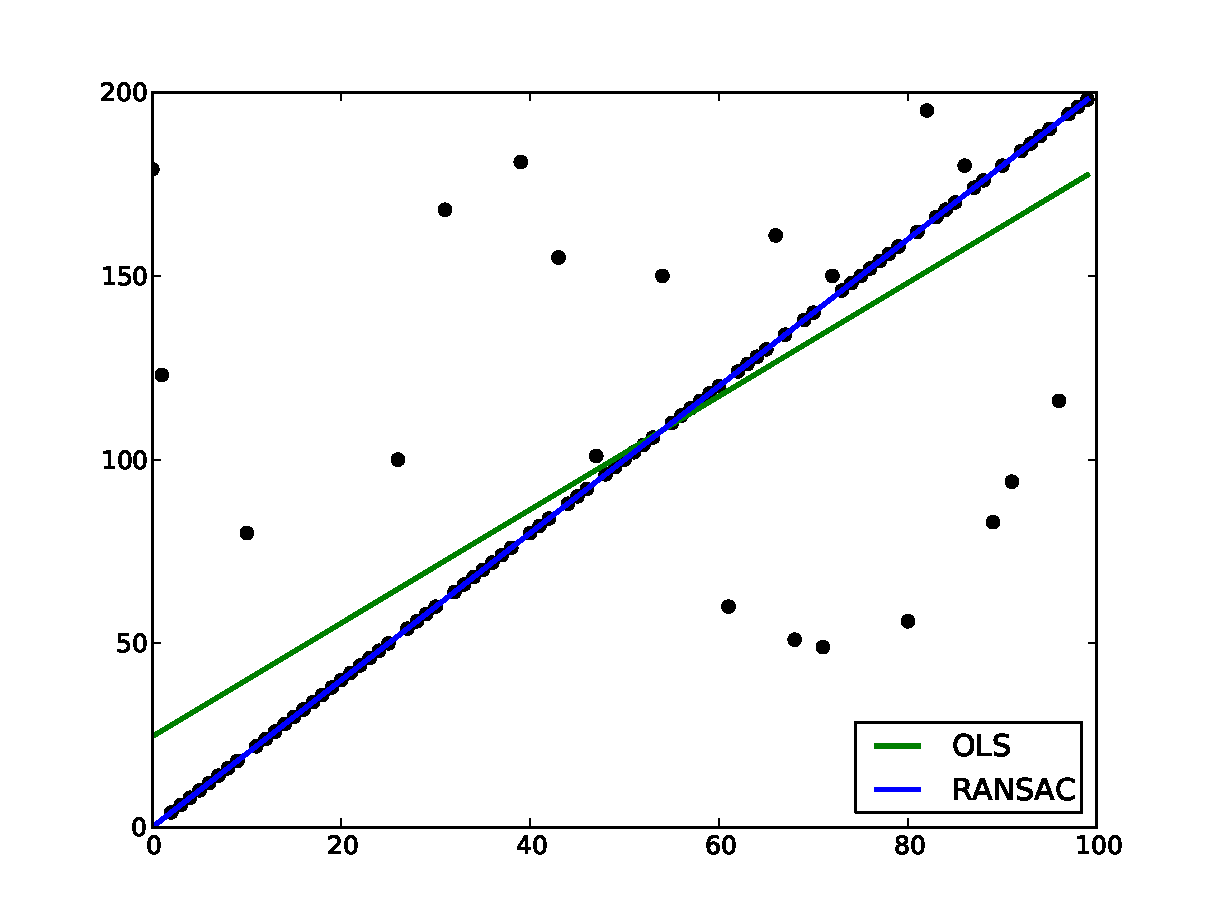
\includegraphics[height=4cm]{img/ransac.pdf}\\
                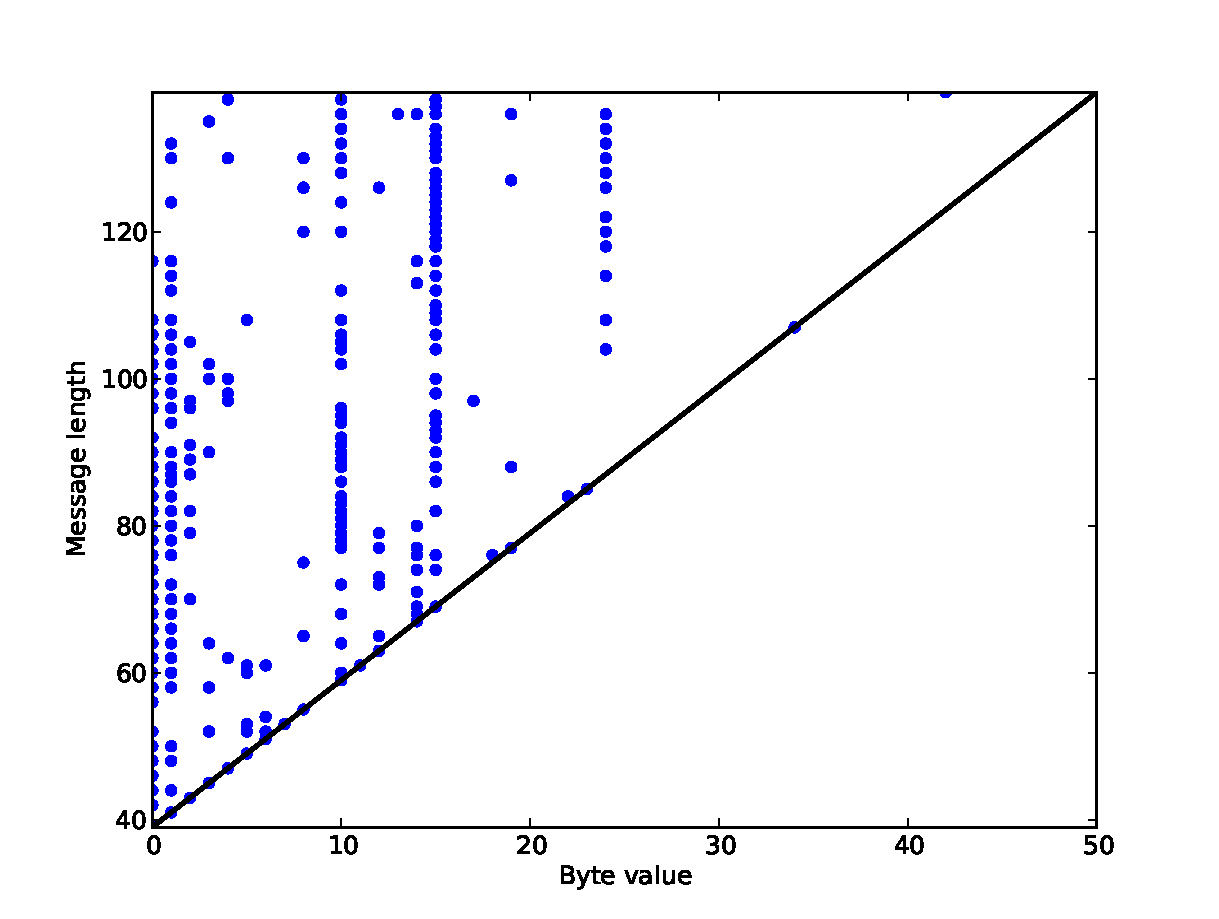
\includegraphics[height=4cm]{img/length.pdf}
            \end{column}
        \end{columns}
    \end{frame}

    % Tillstånd
    \begin{frame}
        \frametitle{Protokolls tillstånd}
        \begin{itemize}
            \item Protokoll modelleras ofta efter \emph{tillståndsdiagram}
            \item Vet vilka typer som finns och i vilken ordning de skickats
            \item Kan delvis återskapa tillståndsdiagrammet
            \item Att återskapa tillståndsdiagrammet för alla tillstånd är
                oftast för rörigt. Nöjer oss med protokollets initiering.
        \end{itemize}
        \begin{columns}[t]
            \begin{column}[T]{5cm}
                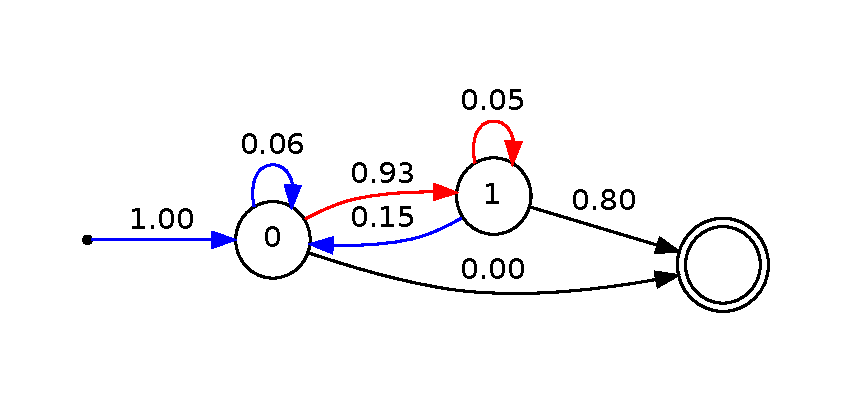
\includegraphics[height=3cm]{img/dnsstate.pdf}
            \end{column}
            \begin{column}[T]{6cm}
                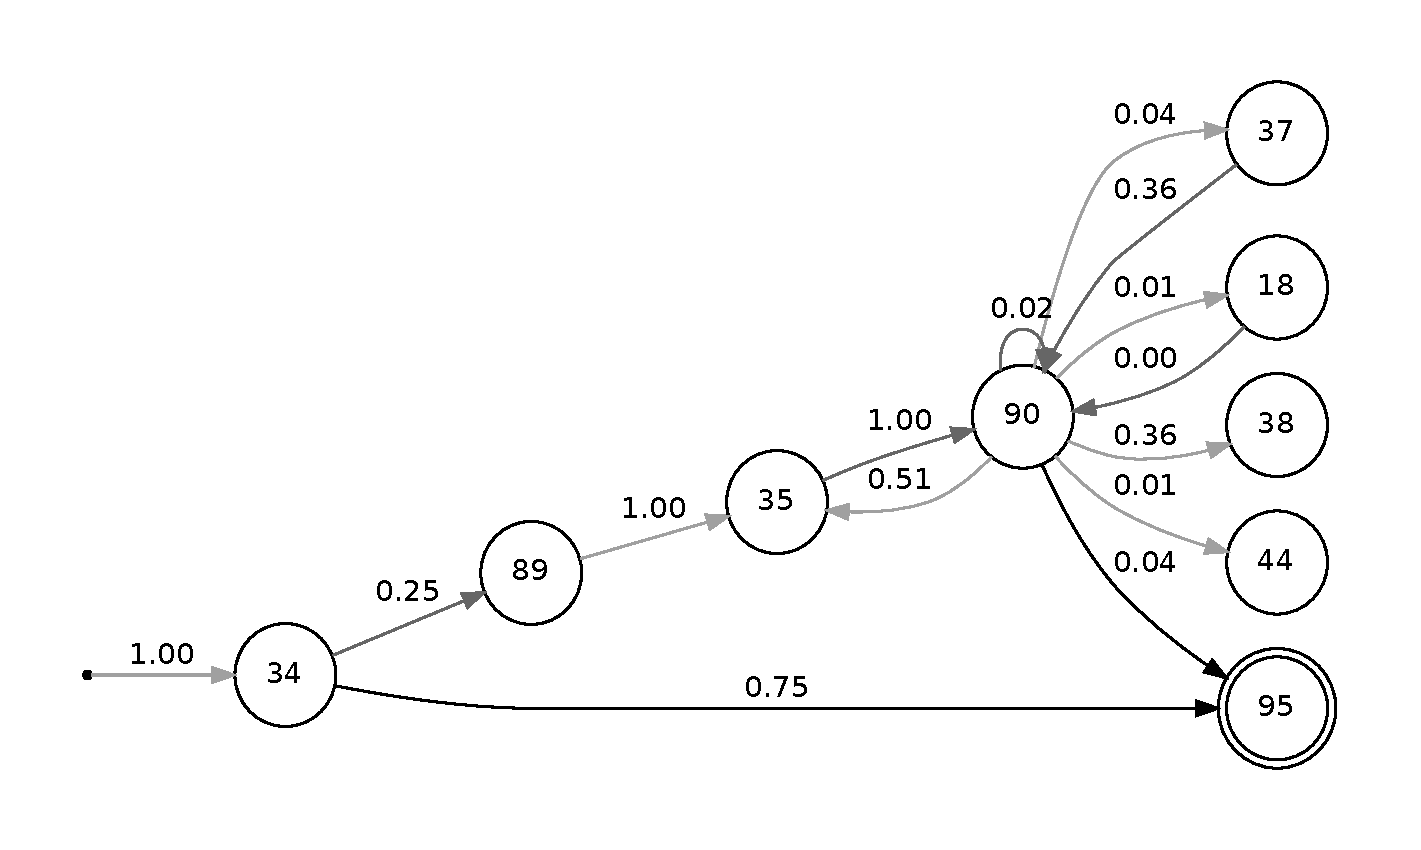
\includegraphics[height=3.5cm]{img/smbstate.pdf}
            \end{column}
        \end{columns}

    \end{frame}

    % Resultat
    \begin{frame}
        \frametitle{Resultat -- Klustring}
        Resultat efter OPTICS:
        \begin{table}[h]
            \centering
            \scriptsize{
                \begin{tabular}{| l | r | r | r | r | r |}
                    \hline
                    \textbf{Protokoll}&\textbf{Completeness}&\textbf{Homogenity}&\textbf{V-measure} \\ \hline
                    DNS & 0.1982 & 0.9550 & 0.3282 \\ \hline
                    SMB & 0.8480 & 0.8632 & 0.8555 \\ \hline
                    TFTP & 0.3015 & 0.9449 & 0.4571 \\ \hline
                    RTP & 0.0000 & 1.0000 & 0.0000 \\ \hline
                    DHCP & 0.3492 & 0.1224 & 0.1813 \\ \hline
                \end{tabular}
            }
        \end{table}
        Resultat efter förfining:
        \begin{table}[h]
            \centering
            \scriptsize{
                \begin{tabular}{| l | r | r | r | r | r |}
                    \hline
                    \textbf{Protokoll}&\textbf{Completeness}&\textbf{Homogenity}&\textbf{V-measure} \\ \hline
                    DNS & 0.9534 & 0.9999 & 0.9761 \\ \hline
                    SMB & 0.9914 & 0.9880 & 0.9897 \\ \hline
                    TFTP & 1.0000 & 1.0000 & 1.0000 \\ \hline
                    RTP & 0.0000 & 1.0000 & 0.0000 \\ \hline
                    DHCP & 1.0000 & 0.4428 & 0.6138 \\ \hline
                \end{tabular}
            }
        \end{table}
    \end{frame}
    \begin{frame}
        \frametitle{Resultat -- Fält}
        \begin{table}[h]
            \scriptsize{
                \begin{tabular}{| l | r | r | r |}
                    \hline
                    \textbf{Protokoll}&\textbf{\# Korrekta Bitar}&\textbf{\# Bitar Totalt}&\textbf{Riktighet (\%)} \\ \hline
                    DNS & 37 & 96 & 38.5 \\ \hline
                    SMB & 112 & 288 & 38.9 \\ \hline
                    TFTP & 0 & 16 & 0.0 \\ \hline
                    RTP & 40 & 96 & 41.7 \\ \hline
                    DHCP & 64 & 1888 & 3.4 \\ \hline
                \end{tabular}
            }
        \end{table}

        Exempel: DNS
        \begin{columns}[t]
            \begin{column}[T]{5cm}
                \begin{bytefield}[bitwidth=0.3cm]{16}
                    \bitheader{0, 16}\\
                    \wordbox{1}{U}\\
                    \bitbox{1}{F}
                    \bitbox{4}{F}
                    \bitbox{1}{F}
                    \bitbox{1}{F}
                    \bitbox{1}{F}
                    \bitbox{1}{F}
                    \bitbox{3}{C}
                    \bitbox{4}{F}\\
                    \wordbox{1}{N}\\
                    \wordbox{1}{N}\\
                    \wordbox{1}{N}\\
                    \wordbox{1}{N}
                \end{bytefield}
            \end{column}
            \begin{column}[T]{5cm}
                \begin{bytefield}[bitwidth=0.3cm]{16}
                    \bitheader{0, 16}\\
                    \wordbox{1}{U}\\
                    \bitbox{8}{SC}
                    \bitbox{8}{F}\\
                    \wordbox{1}{C}\\
                    \bitbox{8}{C}
                    \bitbox{8}{N}\\
                    \bitbox{8}{C}
                    \bitbox{8}{N}\\
                    \bitbox{8}{C}
                    \bitbox{8}{UNK}
                \end{bytefield}
            \end{column}
        \end{columns}
    \end{frame}
    % Begränsningar
    \begin{frame}
        \frametitle{Begränsningar}
        \begin{itemize}
            \item Textuella protokoll
            \item Icke-justerad data
            \item Bit-precision
        \end{itemize}
    \end{frame}

\end{document}
